\section{系统的描述}

系统是由若干个有相互关联的单元组合而成的具有特定功能的整体。

\subsection{系统的分类}

\begin{itemize}
    \item 连续(时间)系统/离散(时间)系统/混合系统(连续和离散系统的组合)
    \item 动态系统/即时系统(记忆/无记忆系统)
\end{itemize}

\subsection{系统的数学模型}

连续系统解析描述:微分方程

离散系统解析描述:差分方程

\subsection{系统的框图描述}

\begin{Figure}[连续系统的基本单元]
    \begin{FigureSub}[加法器]
        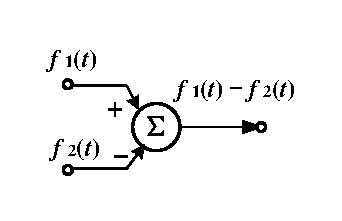
\includegraphics[width=40mm]{visio/1.16-a.pdf}
    \end{FigureSub}
    \begin{FigureSub}[乘法器]
        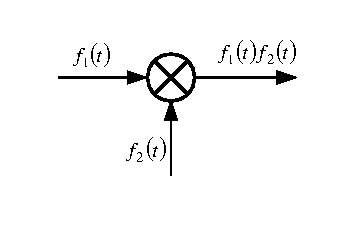
\includegraphics[width=40mm]{visio/1.16-b.pdf}
    \end{FigureSub}
    \begin{FigureSub}[积分器]
        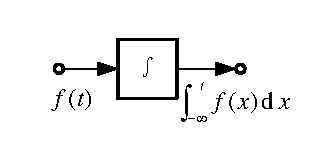
\includegraphics[width=40mm]{visio/1.16-c.pdf}
    \end{FigureSub}
    \begin{FigureSub}[延时器]
        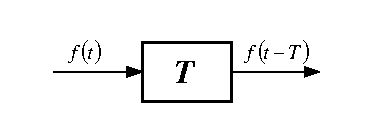
\includegraphics[width=40mm]{visio/1.16-d.pdf}
    \end{FigureSub}
    \begin{FigureSub}[数乘器]
        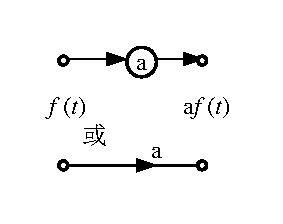
\includegraphics[width=40mm]{visio/1.16-e.pdf}
    \end{FigureSub}
\end{Figure}

微分器用积分器表示

\begin{Figure}[离散系统的基本单元]
    \begin{FigureSub}[离散系统的加法器]
        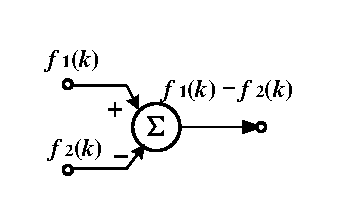
\includegraphics[width=40mm]{visio/1.17-a.pdf}
    \end{FigureSub}
    \begin{FigureSub}[离散系统的延时器]
        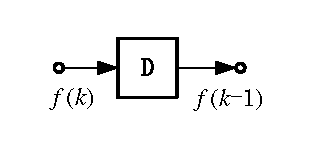
\includegraphics[width=40mm]{visio/1.17-b.pdf}
    \end{FigureSub}
    \begin{FigureSub}[离散系统的数乘器]
        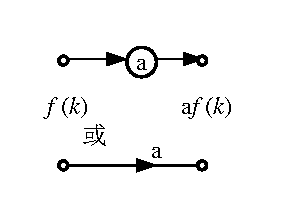
\includegraphics[width=40mm]{visio/1.17-c.pdf}
    \end{FigureSub}
\end{Figure}

根据微分方程画系统框图:

例:$ay''(t)+by'(t)+cy(t) = df'(t)+ef(t)$

设辅助函数$f(t)=ax''(t)+bx'(t)+cx(t)$

\begin{figure}[H]
    \centering
    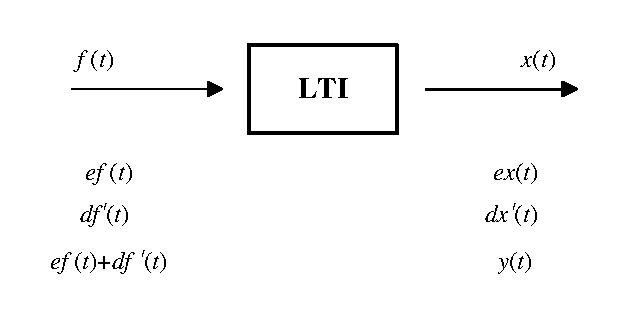
\includegraphics[width=80mm]{visio/sol1.pdf}
\end{figure}

由LTI特性:$y(t)=ex(t)+dx'(t)$

辅助函数移项可得:$x''(t)=f(t)-\frac{b}{a}x'(t)-\frac{c}{a}x(t)$


\begin{figure}[H]
    \centering
    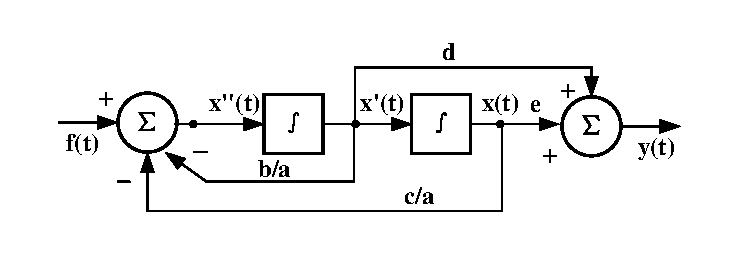
\includegraphics[width=100mm]{visio/sol2.pdf}
\end{figure}

对于框图求微分方程,逆向过程即可



